\documentclass[11pt]{article}

\usepackage[margin=1in]{geometry}
\usepackage{setspace}
\onehalfspacing
\usepackage{graphicx}
\graphicspath{report_images/}
\usepackage{appendix}
\usepackage{listings}
\usepackage{float}

% DOCUMENT INFORMATION =================================================
\title {ECEN 429: Introduction to Digital Systems Design Laboratory \\ North Carolina Agricultural and Technical State University \\ Department of Electrical and Computer Engineering} % Declare Title
\author{Reporter: Nikiyah Beaulah\\ \and Partner: Chris Cannon} % Declare authors
\date{February 8, 2018}
% ======================================================================

\begin{document}

\maketitle % Render Title, Author, and Date

\begin{center}
Lab	2
\end{center}

\pagebreak

\section{Introduction}

\section{Background, Design Solution, and Results}

\subsection{Problem 1 Seven Segment Display}
This problem prompted us to utilize the seven-segment display on the Basys3 board. Our input will be a 3-bit number so that we can provide input from 0-9, which is the range that can be displayed by a single seven-segment display. Seven-segment displays include, fittingly, seven segments. Those segments are conventionally referred to as a-g in accordance with Figure ~\ref{fig:sevenSegMap}.

\begin{figure}[h]
\begin{center}
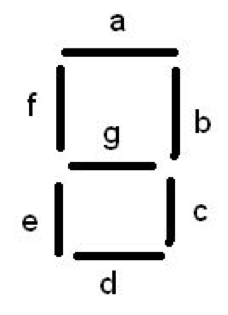
\includegraphics[width=0.2\textwidth]{report-images/img1.png}
\caption{Seven-Segment Display Map}
\label{fig:sevenSegMap}
\end{center}
\end{figure}

\subsubsection{Background}

\subsection{Problem 2 1:2 Decoder}

\subsection{Problem 3 SUM of a Full Adder}

\section{Conclusion}

\end{document}